\documentclass{article}
\usepackage[utf8]{inputenc}
\usepackage[spanish.mexico]{babel}

%\title{Dispositivos}
\author{Pablo Vivar Colina}
%\date{Septiembre 2017}

\usepackage{natbib}
\usepackage{graphicx}

\begin{document}

\maketitle

\begin{figure}[h!]
\centering
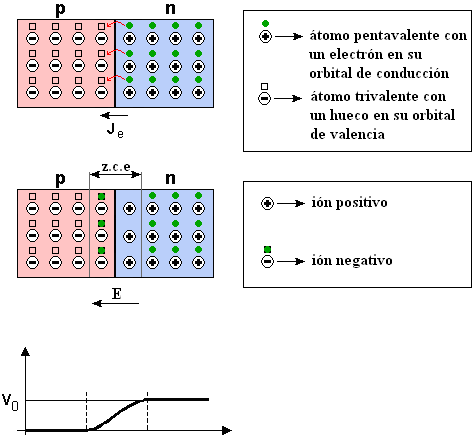
\includegraphics[scale=0.5]{DiodoSem.png}
\caption{Formación de la región de agotamiento, en la gráfica z.c.e.}
\label{fig:diodoSem}
\end{figure}

\begin{figure}[h!]
\centering
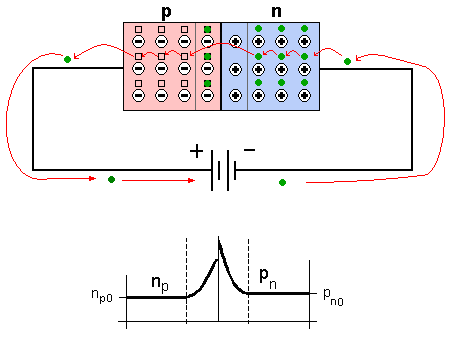
\includegraphics[scale=0.4]{PolDir.png}
\caption{Formación de la región de agotamiento, en la gráfica z.c.e.}
\label{fig:diodoDir}
\end{figure}

\begin{figure}[h!]
\centering
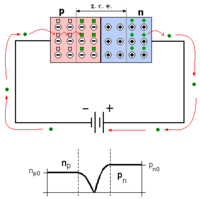
\includegraphics[scale=0.7]{PolInv.png}
\caption{Formación de la región de agotamiento, en la gráfica z.c.e.}
\label{fig:diodoInv}
\end{figure}

\end{document}